\mychapter{1}{Assignment 6 \\ \vspace{-0.3cm} Implementing an FCNN from
Scratch using TensorFlow}
\addcontentsline{toc}{chapter}{Assignment 6 Implementing an FCNN from Scratch using TensorFlow}



\section*{Problem Statement: } \\
\item Implement the following computations using TensorFlow:
\begin{document}
%\thispagestyle{bordered}


\begin{enumerate}
    \item  Load the the MNIST dataset from tensorflow as x train, y train, x test and y test.
The Modified National Institute of Standards and Technology (MNIST) dataset
contains grayscale images of handwritten digits. The training set consists of 60,000
images and the test set contains 10,000 images. The label of each image is a digit
between 0 and 9. Each image has a size of 28 × 28, consisting of 784 pixel values,
where each pixel value ∈ [0, 255] with 0 corresponds to black, 255 to white, and
values in between representing various shades of gray.
    \item Compute X as the transpose of U.

    \item Normalize the pixel values of X to [0, 1] by dividing by 255.

    \item Form a matrix Y of size m corresponding to the labels ∈ [0, 9] of images by transposing y train.

    \item Form a matrix V by reshaping the images in x test to be 1D arrays of 784 (28 × 28)
pixel values (Flatten the images).

    \item Compute Xtest as the transpose of V .

    \item Normalize the pixel values of Xtest to [0, 1] by dividing by 255.

    \item Form a matrix Y test of size m corresponding to the labels ∈ [0, 9] of images by
transposing y test.

    \item Select an image from X and display it. Also, display the corresponding label from
Y.

    \item Form a matrix Y of size m corresponding to the labels ∈ [0, 9] of images by transposing y train.

    \item Set the hyper parameters: p = 10, the no. of neurons in hidden layer, q = 10,
the no. of neurons in output layer (corresponding 10 labels in one-hot encoding
format), learning rate α = 0.01 and the number of training epochs (iterations over
the dataset) as 1000.

    \item Create a matrix W1 of shape (p, n) and initialize it as W1 = N (0, 1) ×
q
1
n
, where
N (0, 1) represents a matrix of random values drawn from a normal distribution with
mean 0 and standard deviation 1.

    \item Initialize the vector B1 of shape (p, 1) to zeros.

    \item Initialize the matrix $W_2$ of shape $(q, p)$ as $W_2 = \mathcal{N}(0, 1) \times \frac{q_1}{p}$.

    \item Initialize the vector B2 of shape (q, 1) to zeros.

    \item Perform the following forward propagation and backpropagation computations iteratively (No. of epochs=1000):
        \begin{enumerate}
        \item  Z1 = W1 · X + B1 (Matrix Multiplication)
        \item A1 = ReLU(Z1) where ReLU(x) is a function that returns 0 for negative values
and the input value itself otherwise.

        \item Z2 = W2 · A1 + B2
        \item $A_2 = \text{softmax}(Z_2)$, where $\text{softmax}(x) = \frac{e^{x_i}}{\sum_j e^{x_j}}$.

        \item Get the predicted labels from the output of A2 (index of the maximum value).

        \item Find the accuracy of the predictions by comparing them to the true labels Y
and print the progress in every 100 epochs.

        \item Compute the cross-entropy loss using TensorFlow’s tf.nn.softmax cross entropy with logits
function.

        \item  dZ2 = A2 − one hot Y where one hot Y is the one-hot encoded form of Y .

        \item $dA_2 = W_2^T \cdot dZ_2$


        \item $dW_2 = \frac{1}{m} \cdot dZ_2 \cdot A_1^T$


        \item $dB_2 = \frac{1}{m} \sum dZ_2 \,\, (\text{sum along the columns})$
 

        \item dZ1 = dA2◦ReLU deriv(Z1) where ReLU deriv(x) returns 1 for positive values
and 0 otherwise, and ◦ indicates element-wise multiplication.

        \item $dA_1 = W_1^T \cdot dZ_1$

        \item $dB_1 = \frac{1}{m} \sum dZ_1 \quad \text{(sum along the columns)}$

        \item $dW_1 = \frac{1}{m} \cdot dZ_1 \cdot X^T$

        \item (p) Update and print $W_1$, $B_1$, $W_2$, and $B_2$ for $\alpha = 0.01$:
            \begin{enumerate}[i.]
                \item $W_1 = W_1 - \alpha \cdot dW_1$
                \item $B_1 = B_1 - \alpha \cdot dB_1$
                \item $W_2 = W_2 - \alpha \cdot dW_2$
                \item $B_2 = B_2 - \alpha \cdot dB_2$
            \end{enumerate}
       \end{enumerate}

       \item . Use tensorflow GradientTape() to automatically calculate the gradients from steps
(h) to (o) and redo the training steps.

        \item Select one test image from Xtest, display it, reshape it to n × 1, perform forward
propagation computations and predict the label. Check whether the prediction is
correct.

    \item Use the entire Xtest and perform the forward propagation computations and predict
the accuracy of the model.

\end{enumerate}

\newpage

\vspace{-.15cm}
\section{Load and Preprocess Data}
\vspace{-.75cm}
\begin{code}
\begin{lstlisting}
import numpy as np
from matplotlib import pyplot as plt
import tensorflow as tf
(x_train, y_train), (x_test, y_test) = tf.keras.datasets.mnist.load_data()
U = tf.reshape(x_train, (x_train.shape[0], 784))
X = tf.transpose(U)
X = tf.cast(X, tf.float32) / 255.0
Y = tf.transpose(tf.convert_to_tensor(y_train))
n, m = X.shape
V = tf.reshape(x_test, (x_test.shape[0], 784))
Xtest = tf.transpose(V)
Xtest = tf.cast(Xtest, tf.float32) / 255.0
Ytest = tf.transpose(tf.convert_to_tensor(y_test))
\end{lstlisting}
\end{code}
\vspace{-1cm}
\begin{verbatim} 
Downloading data from https://storage.googleapis.com/tensorflow/tf-keras-datasets/mnist.npz
11490434/11490434 0s 0us/step

\end{verbatim}
\vspace{-.6cm}
\section{ Display an Image}
\vspace{-.75cm}
\begin{code}
\begin{lstlisting}
ind = 0
image = X[:, ind]
image = tf.reshape(image, (28, 28)) * 255
image_np = image.numpy()
plt.imshow(image_np, cmap='gray', interpolation='nearest')
print(f"Label: {Y[ind].numpy()}")
plt.show()
\end{lstlisting}
\end{code}
\vspace{-1cm}
    \begin{figure}[h!]
        \centering
        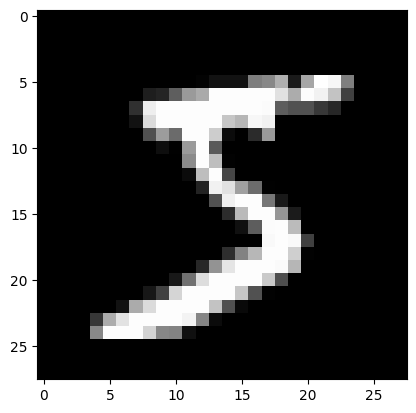
\includegraphics[width=8cm, height=8cm]{ass6pic.png}
        \caption{Image Visualization}
        \label{fig:image_visualization}
    \end{figure}         

    \vspace{-.3cm}

\newpage
\vspace{-.3cm}
\section{Neural Network Parameters}
\vspace{-.9cm}
\begin{code}
\begin{lstlisting}
p = 10
c = 10
alpha = 0.01
epoch = 1000
W1 = tf.Variable(tf.random.normal((p, n), stddev=tf.math.sqrt(1. / n)))
b1 = tf.Variable(tf.zeros((p, 1)))
W2 = tf.Variable(tf.random.normal((c, p), stddev=tf.math.sqrt(1. / p)))
b2 = tf.Variable(tf.zeros((c, 1)))  
\end{lstlisting}
\end{code}

\vspace{-1cm}
\begin{verbatim}
\end{verbatim}

\vspace{-.75cm}
\section{ Activation Functions and Encoding}
\vspace{-.6cm}
\begin{code}
\begin{lstlisting}
def ReLU(Z):
return tf.maximum(Z, 0)
def ReLU_deriv(Z):
return tf.cast(Z > 0, dtype=tf.float32)
def softmax(Z):
exp_Z = tf.exp(Z - tf.reduce_max(Z))
return exp_Z / tf.reduce_sum(exp_Z, axis=0, keepdims=True)
def one_hot(Y):
return tf.one_hot(Y, depth=tf.reduce_max(Y) + 1)
\end{lstlisting}
\end{code}
\vspace{-.75cm}
\begin{verbatim}

\end{verbatim}
\vspace{-.75cm}
\section{Training Loop}
\vspace{-.6cm}
\begin{code}
\begin{lstlisting}
for i in range(epoch):
Z1 = tf.matmul(W1, X) + b1
A1 = ReLU(Z1)
Z2 = tf.matmul(W2, A1) + b2
A2 = softmax(Z2)
one_hot_Y = one_hot(tf.cast(Y, dtype=tf.int32))
one_hot_Y = tf.transpose(one_hot_Y)
if i % 100 == 0:
yhat = tf.argmax(A2, axis=0)
accuracy=tf.reduce_mean(tf.cast(yhat==tf.cast(Y,dtype=tf.int64),dtype=tf.float32)).numpy() * 100
print(f"Epoch: {i}, Accuracy: {accuracy:.2f}%")
\end{lstlisting}
\end{code}
\begin{code}
\begin{lstlisting}
dZ2 = A2 - one_hot_Y
dW2 = 1 / m * tf.matmul(dZ2, tf.transpose(A1))
db2 = 1 / m * tf.reduce_sum(dZ2, axis=1, keepdims=True)
dA2 = tf.matmul(tf.transpose(W2), dZ2)
dZ1 = dA2 * ReLU_deriv(Z1)
dW1 = 1 / m * tf.matmul(dZ1, tf.transpose(X))
db1 = 1 / m * tf.reduce_sum(dZ1, axis=1, keepdims=True)
W2.assign(W2 - alpha * dW2)
b2.assign(b2 - alpha * db2)
W1.assign(W1 - alpha * dW1)
b1.assign(b1 - alpha * db1)
\end{lstlisting}
\end{code}
\vspace{-1cm}
\begin{verbatim}







Epoch: 0, Accuracy: 7.20%
Epoch: 100, Accuracy: 31.82%
Epoch: 200, Accuracy: 47.35%
Epoch: 300, Accuracy: 66.75%
Epoch: 400, Accuracy: 74.39%
Epoch: 500, Accuracy: 78.53%
Epoch: 600, Accuracy: 80.75%
Epoch: 700, Accuracy: 82.20%
Epoch: 800, Accuracy: 83.30%
Epoch: 900, Accuracy: 84.22%
\end{verbatim}
%\vspace{-.6cm}
%\newpage
\section{Make Predictions}
\begin{lstlisting}
def show_prediction(index, W1, b1, W2, b2):
testimage = Xtest[:, index]
testimage = tf.reshape(testimage, (784, 1))
Z1 = tf.matmul(W1, testimage) + b1
A1 = ReLU(Z1)
Z2 = tf.matmul(W2, A1) + b2
A2 = softmax(Z2)
yhat = tf.argmax(A2, axis=0).numpy()
label = Ytest[index].numpy()
testimage = tf.reshape(testimage, (28, 28)) * 255
plt.gray()
plt.imshow(testimage, interpolation='nearest')
plt.show()
print("Prediction:", yhat)
print("Actual Label:", label)
index=39
show_prediction(index, W1, b1, W2, b2)
\end{lstlisting}


\vspace{-1cm}
    \begin{figure}[h!]
        \centering
        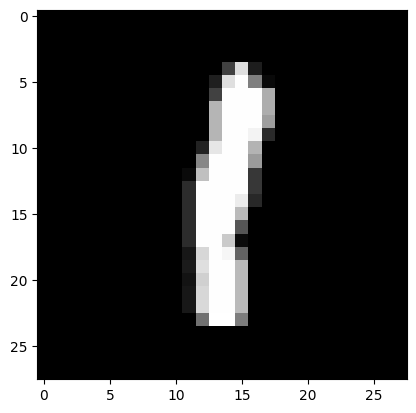
\includegraphics[width=8cm, height=8cm]{ass6pic2.png}
        \caption{Image Visualization}
        \label{fig:image_visualization}
    \end{figure}         

    \vspace{-.3cm}  

\section{Evaluate Model}
\begin{lstlisting}
def test(Xtest, Ytest, W1, b1, W2, b2):
Z1 = tf.matmul(W1, Xtest) + b1
A1 = ReLU(Z1)
Z2 = tf.matmul(W2, A1) + b2
A2 = softmax(Z2)
yhat = tf.argmax(A2, axis=0).numpy()
accu = tf.reduce_mean(tf.cast(tf.equal(yhat, Ytest), dtype=tf.float32)).numpy() * 100
print("Predictions:", yhat)
print("Actual Labels:", Ytest.numpy())
print("Accuracy:", accu, "%")
test(Xtest,Ytest,W1,b1,W2,b2)
\end{lstlisting}
\begin{verbatim}
 Predictions: [7 2 1 ... 4 8 6]
Actual Labels: [7 2 1 ... 4 5 6]
Accuracy: 85.6000006198883 %
\end{verbatim}
\newpage
\section{Error, Precision, Recall,f1 score}
\begin{lstlisting}
from sklearn.metrics import confusion_matrix, precision_score, recall_score, f1_score
def test_and_evaluate(Xtest, Ytest, W1, b1, W2, b2):
Z1 = tf.matmul(W1, Xtest) + b1
A1 = ReLU(Z1)
Z2 = tf.matmul(W2, A1) + b2
A2 = softmax(Z2)
yhat = tf.argmax(A2, axis=0).numpy()
y_true = Ytest.numpy()
cm = confusion_matrix(y_true, yhat)
error_rate = 1 - np.trace(cm) / np.sum(cm)
precision = precision_score(y_true, yhat, average='weighted')
recall = recall_score(y_true, yhat, average='weighted')
f1 = f1_score(y_true, yhat, average='weighted')
print("Confusion Matrix:\n", cm)
print("Error Rate:", error_rate)
print("Precision:", precision)
print("Recall:", recall)
print("F1 Score:", f1)
test_and_evaluate(Xtest, Ytest, W1, b1, W2, b2)
\end{lstlisting}
\begin{verbatim}              
Confusion Matrix:
[[ 935 0 2 6 1 8 17 2 9 0]
[ 0 1103 2 5 1 0 4 1 19 0]
[ 18 23 849 50 20 1 29 19 19 4]
[ 10 6 35 839 2 45 7 10 38 18]
[ 1 9 6 0 831 2 13 0 12 108]
[ 24 15 7 95 30 634 24 15 32 16]
[ 24 8 7 0 13 20 877 0 9 0]
[ 8 41 28 3 9 1 1 881 12 44]
[ 5 29 8 38 23 25 14 19 795 18]
[ 10 11 9 7 94 20 1 26 15 816]]
Error Rate: 0.14400000000000002
Precision: 0.8560334612260678
Recall: 0.856
F1 Score: 0.8549597853086216
\end{verbatim}